\documentclass{beamer}
\usepackage{tikz}
\title{Introduction to Binary Exploitation (and its relevance to Servo) - RCOS Presentation}
\date{November 6, 2015}
\author{Avi Weinstock}
\usepackage{fancyvrb}
\begin{document}
\maketitle

\begin{frame}[fragile]
\frametitle{Trusted vs. Untrusted input}
\begin{itemize}
\item
Trusted input
\begin{Verbatim}[frame=single]
# Don't actually run these, they're dangerous
rm -rf --no-preserve-root /
dd if=/dev/urandom of=/dev/sda bs=4096
\end{Verbatim}
\item
Untrusted input\footnote{\Verb|https://xkcd.com/327/|}
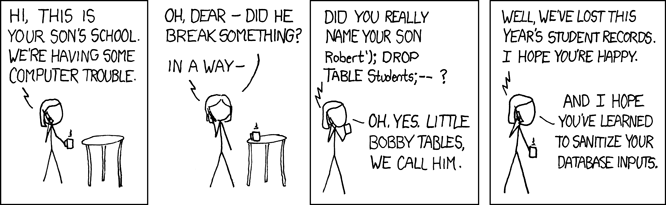
\includegraphics[width=0.8\textwidth]{xkcd_sqli.png}
\end{itemize}
\end{frame}

\begin{frame}[fragile]
\frametitle{Basic memory corruption}
\verb|ssh narnia0@narnia.labs.overthewire.org|\\
\begin{Verbatim}[frame=single, fontsize=\scriptsize]
#include <stdio.h>
#include <stdlib.h>

int main(){
        long val=0x41414141;
        char buf[20];

        printf("Correct val's value from 0x41414141 -> 0xdeadbeef!\n");
        printf("Here is your chance: ");
        scanf("%24s",&buf);

        printf("buf: %s\n",buf);
        printf("val: 0x%08x\n",val);

        if(val==0xdeadbeef)
                system("/bin/sh");
        else {
                printf("WAY OFF!!!!\n");
                exit(1);
        }

        return 0;
}
\end{Verbatim}
\end{frame}

\begin{frame}[fragile]
\frametitle{Shellcode}
\begin{Verbatim}[frame=single, fontsize=\scriptsize]
# grep execve /usr/include/x86_64-linux-gnu/asm/unistd_32.h
# #define __NR_execve		 11
# man 2 execve
# int execve(const char *filename, char *const argv[], char *const envp[]);
# https://en.wikibooks.org/wiki/X86_Assembly/Interfacing_with_Linux
# eax = syscall[eax](ebx, ecx, edx, esi, edi, ebp)
xor %eax, %eax
xor %ecx, %ecx
xor %edx, %edx
mov $11, %al
jmp strLiteral
afterStrLiteral:
pop %ebx
int $0x80
strLiteral:
call afterStrLiteral
.string "/bin/sh"
\end{Verbatim}
\begin{Verbatim}[frame=single, fontsize=\scriptsize]
const char main[] =
    "\x31\xc0\x31\xc9\x31\xd2\xb0\x0b\xeb\x03\x5b\xcd\x80"
    "\xe8\xf8\xff\xff\xff\x2f\x62\x69\x6e\x2f\x73\x68\x00";
\end{Verbatim}
\end{frame}

\begin{frame}[fragile]
\frametitle{Use of shellcode}
\verb|ssh narnia1@narnia.labs.overthewire.org|\\
\begin{Verbatim}[frame=single, fontsize=\scriptsize]
#include <stdio.h>

int main(){
        int (*ret)();

        if(getenv("EGG")==NULL){
                printf("Give me something to execute"
                       " at the env-variable EGG\n");
                exit(1);
        }

        printf("Trying to execute EGG!\n");
        ret = getenv("EGG");
        ret();

        return 0;
}
\end{Verbatim}
\end{frame}

\begin{frame}[fragile]
\frametitle{Injecting shellcode}
\verb|ssh narnia2@narnia.labs.overthewire.org|\\
\begin{Verbatim}[frame=single, fontsize=\scriptsize]
#include <stdio.h>
#include <string.h>
#include <stdlib.h>

int main(int argc, char * argv[]){
        char buf[128];

        if(argc == 1){
                printf("Usage: %s argument\n", argv[0]);
                exit(1);
        }
        strcpy(buf,argv[1]);
        printf("%s", buf);

        return 0;
}
\end{Verbatim}
\end{frame}

\begin{frame}[fragile]
\frametitle{Thanksgiving}
\begin{itemize}
\item Professor Goldschmidt
\item Professor Moorthy
\item The Mozilla Project
\item RCOS's current sponsors
\item All of RCOS
\item All of RPISEC
\item \verb|http://overthewire.org/wargames/|
\item Randall Munroe
\end{itemize}
\end{frame}

\end{document}
